\documentclass[11pt]{article}

\setlength\parindent{0pt}
\setlength{\parskip}{.25\baselineskip}

\usepackage{hyperref}
\usepackage{amsmath,amsfonts,amssymb,bbm}
\usepackage{todonotes}

\DeclareMathOperator{\Tr}{Tr}

\newcommand{\R}{\mathbbm{R}}
\newcommand{\mba}{\mathbf{a}}
\newcommand{\mbb}{\mathbf{b}}
\newcommand{\mbx}{\mathbf{x}}
\newcommand{\mbxt}{\tilde{\mathbf{x}}}
\newcommand{\Sigmat}{\tilde{\Sigma}}
\newcommand{\mbz}{\mathbf{z}}
\newcommand{\mbw}{\mathbf{w}}
\newcommand{\mcN}{\mathcal{N}}
\newcommand{\mcP}{\mathcal{P}}
\newcommand{\eps}{\epsilon}
\newcommand{\trans}{\intercal}
\newcommand{\Ut}{\tilde{U}}
\DeclareMathOperator*{\argmax}{arg\,max}

\title{Methods for Astronomical Source Discovery and Separation}
\author{}
\date{\today}

%% DOC START
\begin{document}
\maketitle

The goal of this project is to develop reliable inference techniques to simultaneously discover and characterize properties of distant stars and galaxies from a massive database of photometric imagery.  

We define notation: 
\begin{itemize} \itemsep 0pt
\item $s \in \{1, \dots, S\}$ will index unique sources (stars or galaxies)
\item $n \in \{1, \dots, N\}$ will index unique images
\item $\beta_n \in \{r, \dots, z\}$ will stand for the band of image $n$
\end{itemize}

For each source, we define the following \emph{intrinsic} properties, which are the estimands of interest: 
\begin{align*}
  u_s &= (u_{s,ra}, u_{s,dec}) = \text{right ascension and declination of source $s$} \\
  t_s &= \text{temperature of source $s$ (kelvin)} \\
  d_s &= \text{distance to source $s$ (meters)} \\
  \ell_s &= \text{luminosity of source $s$ (Joules/second)} 
\end{align*}

This paper describes a probabilistic model-based approach to inferring these quantities of interest.  We treat the observed pixel values as random variables, and describe a (stochastic) forward generating procedure based on the properties of these sources (the likelihood), as well as an a priori distribution over the properties themselves (the prior), and use Bayesian inference and Markov Chain Monte Carlo techniques to draw simulations from the posterior.  To understand the likelihood, we first outline the physical motivation underlying our model.  

\section{Computing the expected number of photons}
The random variable that gives rise to our likelihood and motivates probabilistic inference in this problem is the number of photons detected by an instrument with a lens of a fixed area over a fixed exposure duration.  According to our idealized model, this random variable is Poisson distributed conditioned on the intrinsic properties of a source.  To describe our observations, we need to outline the procedure by which the band-specific flux images are generated.  

To compute how many photo-electrons we expect to be captured by a lens of size $A$ over exposure duration $\Delta$, we must compute the number of photons that will eventually be intercepted by the instrument as a function of the source's distance, luminosity, and temperature.  Geometrically, we can view the source as a single point in space at a distance $d_s$, which radiates energy uniformly outward, such that the level sets of equal radiation form a sphere.  We can think of the area of the lens of the instrument as some fraction of the total surface area of this sphere, which is, roughly
\begin{align}
  \frac{A}{4\pi d_s^2} &= \text{ proportion of surface area detected }
\end{align}
If a source is emitting $\ell_s$ Joules per second, the amount of energy that actually is detected by the instrument dissipates as the proportion of surface area decreases, which falls off $\frac{1}{d_s^2}$ as a function of distance (e.g. if we had a `lens' that formed a perfect sphere around the black body, we could effectively measure all $\ell_s \Delta$ Joules for an exposure of length $\Delta$).  

To obtain the total number photo-electrons we expect to detect in band $\beta_n$, we need to compute how much of a black body's energy is distributed within the spectrum recorded by $\beta_n$ \emph{and} account for how our instrument filters $\beta_n$ over a chunk of the energy spectrum (non-uniformly, see Figure~\ref{fig:sensitivity}).

Intuitively, we can do this by computing the photon flux as a function of source temperature and wavelength, and then integrate this value times the sensitivity curve to obtain the total amount of energy we expect the black body to emit per unit area per unit time.  
\begin{align}
  \text{\# P-E detectable in band $\beta_n$} &= I_{\beta_n}(t_s) \cdot \ell_s \frac{A \Delta}{4\pi d_s^2}  
  \label{eq:brightness}
\end{align}
which reads the number of photo-electrons detectable by our instrument in band $\beta_n$ due to a single source $s$ is simply the number of photons we expect to see per unit energy that a source at temperature $t_s$ emits in band $\beta_n$ (modulated by our instrument filter $S_\lambda$) times the total luminosity of the source (energy emitted per second) times the fraction of the sphere at distance $d_s$ we can actually detect times the duration of exposure.  The simple geometric approximation for $\frac{ A \Delta }{ 4 \pi d_s^2 }$ will suffice for that term.  To compute $I_{\beta_n}(t_s)$, we must compute the spectral energy density of an idealized black body, for which we appeal to Planck's law. 

\begin{figure}[t!]
\begin{align*}
  B(t, \lambda) &= \frac{2 h c^2}{\lambda^5} \frac{1}{ e^{\frac{hc}{\lambda k_B t}} - 1} \text{ (Planck's law) } \\
  \int B(t, \lambda) &= P(t) = \frac{\sigma}{\pi} t^4  \text{ (Stefan-Boltzmann) }\\
  E(\lambda) &= \frac{hc}{\lambda} \\
  S(\lambda) &= \text{ instrument sensitivity - lookup table } \\
  A &= \text{ lens area (meters$^2$) } \\
  \Delta  &= \text{ exposure duration (seconds) } \\
  c &= \text{ speed of light (meters / second) } \\
  h &= \text{ Planck constant } \\
  k &= \text{ Boltzmann constant } \\
  \sigma &= \text{ Stefan-Boltzmann constant } 
\end{align*}
\caption{Relevant physical relationships and constants}
\end{figure}

\subsection{Planck's Law}
Our goal is characterize the distribution of energy radiated by an idealized black body as a function of definite temperature and wavelength, which is the relationship described by Planck's law, which tells us that the spectral radiance is given by
\begin{align}
  B(t, \lambda) &= \frac{2 h c^2}{\lambda^5} \frac{1}{ e^{\frac{hc}{\lambda k_B t}} - 1}
\end{align}
which is in units of Watts per steradian per meter$^2$ per wavelength unit.  Intuitively, this describes the amount of energy the black body emits per unit time per unit area per solid angle. 

The total radiance across all wavelengths per square meter per steradian is given by the Stefan-Boltzmann law, which is easily computed as 
\begin{align}
  P(t) = \frac{\sigma}{\pi} t^4 \text{  in J / (s $\cdot$ m$^2$ $\cdot$ str) } 
\end{align}
which is obtainable if you integrate the relationship in Planck's law over wavelength.  Simply dividing the two relationships gives you the energy density, or the \emph{distribution} of energy over the spectrum you expect the black body to exhibit.  We are interested in actual photon counts, so we will want to include the relationship between energy and photons as wavelength varies, given by 
\begin{align}
  E(\lambda) &= \frac{h c}{\lambda} \text{ in J / photon }
\end{align}
Now we must consider the sensitivity of our instrument with respect to wavelength, which allows us to compute our per-wavelength photo-electron fluxes (counts per unit time) as 
\begin{align}
  F(t, \lambda) &= \frac{B(t, \lambda)}{P(t)} \frac{S_{\beta_n}(\lambda)}{E(\lambda)} 
\end{align}
where $S_{\beta_n}(\lambda)$ is the sensitivity filter for band $\beta_n$, which is a function of $\lambda$ with range in the unit interval.  The above value is the number of photons detectable by our sensor per unit wavelength.  

Finally, integrating over wavelength (which will be approximated numerically) will yield the expected number of photo-electrons detected by our instrument in a given band from a source 
\begin{align}
  I_{\beta_n}(t_s) &= \int_{\beta_n} \frac{B(t_s, \lambda)}{P(t_s)} \frac{S_{\beta_n}(\lambda)}{ E(\lambda)} d\lambda
  \label{eq:photojoules}
\end{align}
which gives us the number of photo-electrons per Joule we expect to see from the source in band $\beta_n$.  This is \emph{almost} the random variable we actually observe.  These photo-electrons are then spread out by the instrument according to a calibrated point-spread function (PSF).  The PSF model is known, and will finally relate the observed pixel values to the source's intrinsic properties. 

We can express the numerical integration as a dot product
\begin{align}
  \hat I_{\beta_n}(t_s) &= \mathbf{f}_{t_s}^\trans \mathbf{h_{\beta_n}} \\
  \mathbf{f}_{t_s}     &= (B(t_s, \lambda_1)/P(t_s), \dots, B(t_s, \lambda_L)/P(t_s)) \\ 
  \mathbf{h}_{\beta_n} &= (S_{\beta_n}(\lambda_1)d\lambda / E(\lambda_1), \dots, S_{\beta_n}(\lambda_L)d\lambda / E_{\lambda_L}) 
\end{align}
where $\mathbf{f}_{t_s}$ is the vector approximation to the spectral density of a black body at temperature $t_s$, and $\mathbf{h}_{\beta_n}$ is the vector approximation of the 
which will be a convenient representation when we differentiate the likelihood with respect to $t_s$.  

\subsection{Putting it together}
We can now compute the number of photons from a source as observed in an image by combining Equation~\ref{eq:brightness} with Equation~\ref{eq:photojoules} to yield
\begin{align}
  c(t_s, d_s, \ell_s, \beta_n) &= 
    \underbrace{I_{\beta_n}(t_s, S_\lambda)}_{
      \substack{ \text{\# photons detectable} \\
                 \text{in band $\beta_n$ from a } \\
                 \text{source at temp} \\
                 \text{$t_s$ per Joule}}} \cdot 
    \underbrace{ \ell_s }_{
      \substack{ \text{ Joules/sec } \\
                 \text{ radiated by} \\
                 \text{ source $s$ } }} \cdot
    \underbrace{ \frac{A}{4\pi d_s^2} }_{
      \substack{ \text{ proportion of } \\
                 \text{ sphere measurable } \\
                 \text{ by instrument }}} \cdot
    \underbrace{ \Delta }_{
      \substack{ \text{ exposure } \\
                 \text{ duration (s) } } }
\end{align}
giving us the expected number of photons that source $s$ contributes to image $n$.  

\begin{figure}[t!]
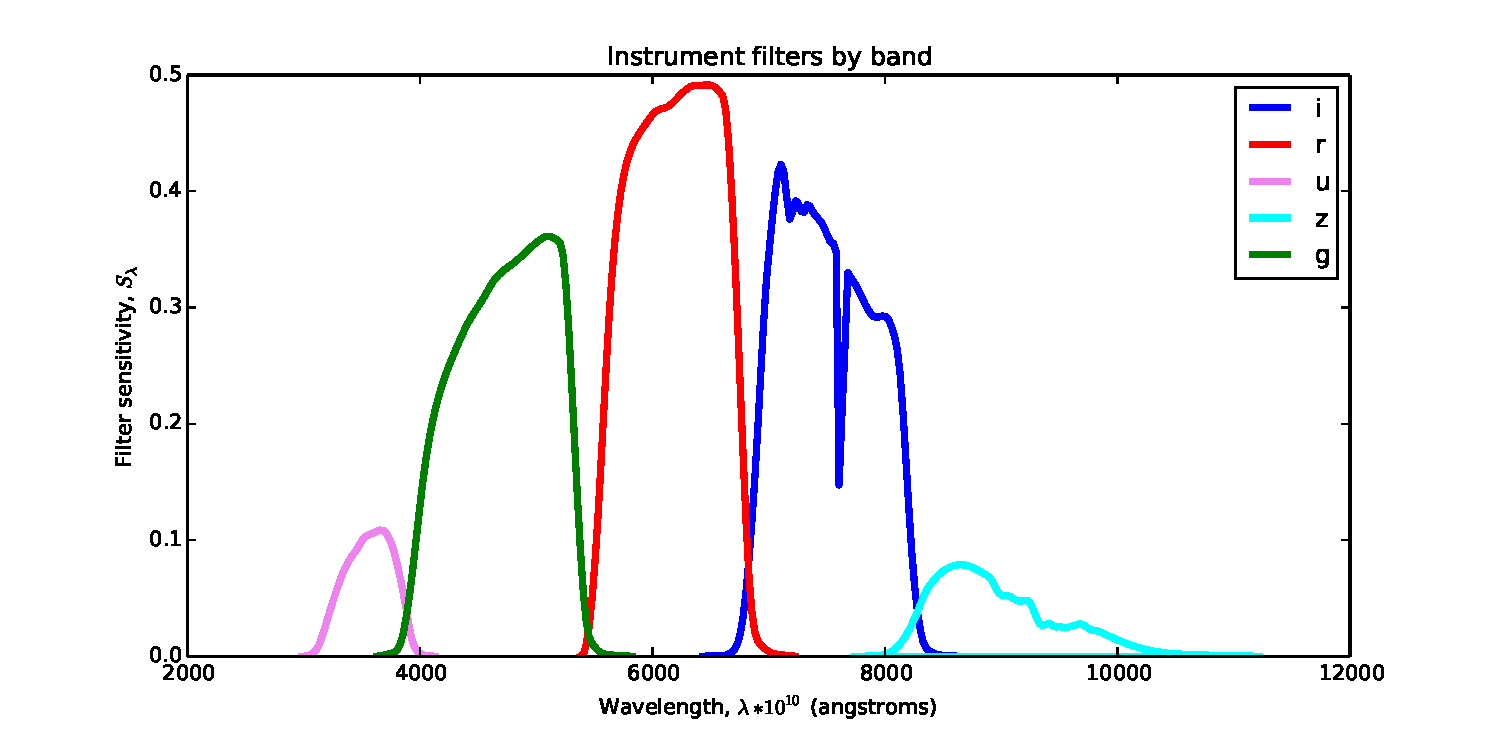
\includegraphics[width=\textwidth]{imgs/filter_sensitivity.pdf}
\caption{Instrument filter sensitivity curves in each band.  The amount of energy (i.e. number of photo-electrons detected) are are not collected uniformly across the range of wavelengths detected in each band - they are scaled according to these curves.  The total count for each band will be the integral of number of photo-electrons detected in each wavelength (energy level), scaled by these curves. }
\label{fig:sensitivity}
\end{figure}


\section{From Sources to Pixel Observations}
An image $n$ corresponds to measurements in one band, $\beta_n$, and consists of pixels locations denoted by $m = (w,h)$.  The total number of photons we expect to observe in image $n$ is simply the sum of the contribution we expect to see from each source, described above.  However, this total number is distributed about the pixels of the image according to the image's point spread function (PSF), due to atmospheric turbulence.  For image $n$ (with only point source contributions) and pixel $m = (w,h)$, the distribution over photon count is modeled
\begin{align}
  x_{n,m} | \{(u_s, t_s, \ell_s, d_s)\}_{s=1}^S &\sim \textrm{Poisson}( F_{n,m} ) \\
  F_{n,m} &= \epsilon_n + \sum_{s=1}^S \underbrace{c(t_s, d_s, \ell_s, \beta_n) f_s(m)}_{\equiv F_{n,m,s}} \\
  \epsilon_n &\sim \textrm{Gamma}(\alpha, \beta) \\
  c(t_s, d_s, \ell_s, \beta_n) &= \mathbf{f}_{t_s}^\trans \mathbf{h_{\beta_n}} \cdot \ell_s \frac{A \Delta}{4\pi d_s^2}  \\
  f_s(m)  &= \sum_{k=1}^3 w_{n,k} \phi(m; v_{n,s} + \mu_{n,k}, \Sigma_{n,k}) \\
  v_{n,s} &= \Upsilon_n(u_s - \phi_n) + \rho_n
\end{align}
where 
\begin{itemize}
  \item $w_{n,k}, \mu_{n,k}, \Sigma_{n,k}$ for $k=1,2,3$ parameterizes image $n$'s point spread function (PSF) in pixel coordinates
  \item $f_s(m)$ is the amount of the source that is assigned to pixel $m$ (the PSF itself)
  \item $\epsilon_n$ acts as a bias term, explaining counts unexplained by sources in image $n$ 
  \item $v_{n,s}$ is the location of the source in pixel coordinates, an image-specific linear transformation of $u_s$. 
\end{itemize}
Due to an identifiability issue, we can only infer the ratio of $\ell_s$ and $d_s^2$, which we instead parameterize it's \emph{apparent brightness} (measured in Joules per meter$^2$ second)
\begin{align}
  b_s \equiv \frac{\ell_s}{4 \pi d_s^2}
\end{align}

We can write the likelihood as 
\begin{align}
   L(\{u_s, t_s, b_s\}_{s=1}^S)
     &= \prod_{n=1}^N \prod_{m \in \mathcal{P}_n} p_{pois}(x_{n,m} ; F_{n,m}) \\
     &= \prod_{n,m} \frac{ F_{n,m}^{x_{n,m}}}{x_{n,m}!} e^{-F_{n,m}}
\end{align}
where $\mathcal{P}_n$ denotes the set of pixels in image $n$.  

and the log likelihood, over all images, as 
\begin{align}
  \log L(\{u_s, t_s, b_s\}_{s=1}^S) 
    &= \underbrace{\sum_{n=1}^N}_{\text{images}}
       \underbrace{\sum_{m \in \mathcal{P}_n}}_{\text{pixels in $n$}}
       \log p_{pois}(x_{n,m}; F_{n,m}) \\
    &= \sum_{n,m} x_{n,m} \log F_{n,m} - F_{n,m} + const.
\end{align}
One problematic aspect of the likelihood is the $\log F_{n,m}$ term, which is difficult to directly optimize and compute with multiple cores.  We can simplify this by using a natural latent variable representation of additive Poisson intensity functions.  

\section{Latent variable representation}
A convenient property of Poisson random variables with additive intensity functions is that they can be viewed as independent Poisson random variables that have been summed, that is
\begin{align}
  X &\sim \textrm{Poisson}(\lambda_1 + \lambda_2 + \dots + \lambda_S) \\
  X_s &\sim \textrm{Poisson}(\lambda_s) \text{ independent for } s = 1, \dots, S \\
  \implies
  X &\sim \sum_{s=1}^S X_s
\end{align}
So we can represent a Poisson random variable, $X$, as the sum of $S$ Poisson random variables, each corresponding to a piece of the original intensity function.  This is a convenient representation if those additive pieces of the intensity function have a useful interpretation, such as photon contribution from individual sources.  Given the sum of $S$ Poisson random variables, the individual components, $X_1, \dots, X_S$ have a multinomial distribution 
\begin{align}
  X_1, \dots, X_s | X=x &\sim \textrm{Mult}\left(n=x, p= \frac{\lambda_1}{\sum \lambda_s}, \dots, \frac{\lambda_S}{\sum \lambda_s} \right) 
\end{align}

We can adopt this latent variable representation in the generative image model.  For each pixel we introduce the latent variables
\begin{align}
 Z_{n,m} = (Z_{n,m,0}, Z_{n,m,1}, \dots, Z_{n,m,S})
\end{align}
where each component can be interpreted as the number of photons observed in pixel $m$ of image $n$ due to source $s$, and $Z_{n,m,0}$ is reserved for the background photons.  

Conditioned on $\{Z_{n,m}\}$, we can re-write the likelihood as 
\begin{align}
  L(\{u_s, t_s, b_s\}_{s=1}^S; \{z\})
     &= \prod_{n=1}^N \prod_{m \in \mathcal{P}_n} \prod_{s=0}^S  p_{pois}(z_{n,m,s} ; F_{n,m, s}) 
\end{align}
where we define $F_{n,m,0} \equiv \epsilon_n$.  For an image $n$ and a source $s$, we can gather all photons assigned to that source add them
\begin{align}
  z_{n,m,s} &\sim \textrm{Pois}(F_{n,m,s}) \\
  \sum_{m} z_{n,m,s} &\sim \textrm{Pois}\left( \sum_{m} F_{n,m} \right) \\
    &\sim \begin{cases}
         \textrm{Pois}( c(t_s, d_s, \ell_s, \beta_n) ) & \text{ if } s > 0  \\
         \textrm{Pois}( M_n \epsilon_n ) & \text{ if } s = 0 
       \end{cases}
\end{align}
which is due to the fact that the PSF is a density, so it sums to one (note that this assumes that image $n$ contains the entire support of the PSF, which will eventually be approximated).  

Conditioning on $Z$ allows us to consider the sources independently.  We can sample each source specific variable, $t_s, b_s$ and $u_s$ independently (and in parallel).  Gibbs sampling strategy then becomes
\begin{itemize}
\item sample $Z_{n,m,s} | X_{n,m}, \{u_s, t_s, b_s\}_{s=1}^S$
\item for each source $s$
  \begin{itemize}
  \item Sample $u_s, t_s, b_s | \{z_{n,m,s}\}_{n=0}^N$
  \end{itemize}
\item Randomly propose a split/merge move: 
  \begin{itemize}
  \item Propose to split source $s$ into two sources, $s_1'$ and $s_2'$.  Accept/reject.
  \item Propose to merge two sources, $s_1$ and $s_2$ into one source, $s'$.  Accept/reject. 
  \end{itemize}
  
\item Randomly propose a birth/death move
  \begin{itemize}
  \item  
  \end{itemize}
\end{itemize}
 
 
\subsection{Sampling source-specific parameters}
Conditioned on the assignment of photons to specific sources, sampling the location, temperature, and brightness variables for a specific source is much simpler.  For a source $s$, we can express the likelihood conditioned on $\{z_{n,m,s}\}$ as 
\begin{align}
  z_{n,m,s} | u_s, t_s, b_s 
    &\sim \textrm{Poisson}(F_{n,m,s}) \\
    &\sim \textrm{Poisson}\left(\mathbf{f}_{t_s}^\trans \mathbf{h}_{\beta_n} \cdot b_s \cdot \frac{A \Delta}{4 \pi} f_s(m) \right)
\end{align}
for $m \in 1, \dots, M_n$ (pixels per image) and $n \in 1, \dots, N$ (total images containing this source).  

The goal is to sample $u_s, t_s, b_s$ leaving the conditional posterior invariant.  Firstly, note that only the location variable $u_s$ relies on the spatial pixel structure through $f_s(m)$.  This allows us to conditionally slice sample these values, and then effectively ignore them (when we sum over the $m$, the $f_s(m)$ term falls out and sums to one).  
\begin{align}
  p(u_s | \{ z_{n,m,s} \}, t_s, b_s) &\propto p( \{ z_{n,m,s} \} | u_s, t_s, b_s) \\
  &= \prod_{m,n} p_{pois}\left(z_{n,m,s}; \mathbf{f}_{t_s}^\trans \mathbf{h}_{\beta_n} \cdot b_s \cdot \frac{A \Delta}{4 \pi} f_s(m) \right)
\end{align}

Conditioned on $u_s$ and $b_s$, we have a somewhat simpler likelihood 
\begin{align}
  p(b_s | \{z_{n,m,s}\}, t_s, u_s) 
    &\propto p_{pois}\left( \sum_{n,m} z_{n,m,s};  \sum_{n} \mathbf{f}_{t_s}^\trans \mathbf{h}_{\beta_n} \cdot b_s \cdot \frac{A \Delta}{4 \pi} \right) 
\end{align}
which gives us a 1-dimensional slice sampling problem.  

Finally, conditioned on $t_s$ and $u_s$, we have a very simple likelihood
\begin{align}
  p(b_s | \{z_{n,m,s}\}, t_s, u_s) 
    &\propto p_{pois}\left( \sum_{n,m} z_{n,m,s}; \sum_{n} \mathbf{f}_{t_s}^\trans \mathbf{h}_{\beta_n} \cdot b_s \cdot \frac{A \Delta}{4 \pi} \right) \\
    &= p_{pois}\left( \sum_{n,m} z_{n,m,s};  b_s C \right)
\end{align}
where $C$ is a constant with respect to the conditional likelihood.  We place a Gamma prior over $b_s$ for conditional conjugacy, admitting a simple posterior sampler. 
\begin{align}
  b_s &\sim \textrm{Gamma}(\alpha_0, \beta_0) \\
  \sum_{n,m} z_{n,m,s} &\sim \textrm{Poisson}(b_s C) \\
  b_s | \{z_{n,m,s}\}, t_s, u_s &\sim \textrm{Gamma}\left(\alpha_0 + \sum_{n,m}z_{n,m,s}, \beta_0 + C\right)
\end{align}


\subsection{Expectation Maximization}
With a fixed number of sources, $S$, the latent variable formulation admits a simple and parallelize-able maximum likelihood procedure.  This can be used as a way to seed the model, or allow us to compute a MAP conditional posterior for particular parameters.  The maximum likelihood procedure is as follows
\begin{itemize}
\item Compute $F_{n,m,s}$ for all $n,m,s$ and define $F_{n,m,0} = \epsilon_n$.  Compute conditional expectations  
\begin{align}
  z_{n,m,s} | u_s, t_s, b_s, x_{n,m,s}
    &\sim \textrm{Mult}(p_{n,m,0}, \dots, p_{n,m,S}; n = x_{n,m})
\end{align}
where 
\begin{align}
  p_{n,m,s} &= \frac{F_{n,m,s}}{\sum_{s=0}^S F_{n,m,s}}
\end{align}

\item The expected complete data log likelihood is
\begin{align}
  E(\ell)
    &= \sum_{n,m,s} E(Z_{n,m,s}) \log F_{n,m,s} - F_{n,m,s} \\
    &= \sum_{n,m,s} x_{n,m} p_{n,m,s} \log F_{n,m,s} - F_{n,m,s} \\
    &= \underbrace{\left( \sum_{n,m} x_{n,m} p_{n,m,0} \log \epsilon_n - \epsilon_n \right)}_{\text{image noise}} + \underbrace{\left(\sum_{n,m,s\neq 0} x_{n,m} p_{n,m,s} \log F_{n,m,s} - F_{n,m,s}\right)}_{\text{source params}}
\end{align}

\item Maximize over source parameters.  Compute
\begin{align}
  \hat \epsilon_n &= \frac{1}{M_n} \sum_{m} x_{n,m} p_{n,m,0} \\
  \hat u_s, \hat b_s, \hat t_s &= \argmax_{u_s, b_s, t_s} \sum_{n,m} x_{n,m} p_{n,m,s} \log F_{n,m,s} - F_{n,m,s}
\end{align}
where the image noise parameters have a straightforward closed form, and the source specific parameters can be optimized numerically.   
\end{itemize}
\todo{Can the source parameters be optimized in a clever way?}

\section{Priors}
For sampling, we must define priors over all of our source and image parameters.  

\begin{align}
  v_s &\propto 1 \\
  t_s &\sim \mathcal{LN}(\tau_1, \tau_2) \\
  b_s &\sim \mathcal{LN}(\gamma_1, \gamma_2) \\
  S   &\sim \textrm{Poisson}(\lambda_n) 
\end{align}


However, we are also free to choose informative priors based on prior knowledge of the joint distribution of the temperatures and luminosities of stars.  For instance, different types of stars exhibit characteristic behavior, such as the stars falling along the main sequence, giants, white dwarfs, etc.  We can encode this prior knowledge by imposing 
\begin{align}
  t_s, b_s &\sim P
\end{align}







\end{document}